\documentclass[12pt]{article}
\usepackage{cite}
\usepackage{graphicx}
\usepackage{subcaption}
\usepackage{caption}
\usepackage{url}

\linespread{1.25} % the equivalent of 1.5 line spacing from msword
\usepackage[a4paper, left=2.5cm,right=2.5cm,top=2.5cm,bottom=2.5cm]{geometry} % margins


\title{Web service workload prediction using deep learning - Report 3}
\date{\today}
\author{Stefan Sebastian}

\begin{document}
  \pagenumbering{gobble}
  \maketitle
  
  \newpage
  \tableofcontents
  \newpage 
  \pagenumbering{arabic}

  \section{State of the art}

  Calheiros et al.\cite{arima_prediction} apply the ARIMA model
  to cloud workload prediction. The model was evaluated using a trace of English Wikipedia resource requests
  spanning a duration of four weeks. The first three are used for training and the fourth for prediction 
  using a time window of 1 hour. The MAPE varies from 9\% to 22\% depending on the confidence interval chosen, 
  from 80 to 95 which is meant to limit the occurences of underestimations.

  Other classic timeseries models have also been applied for this task, like Brown Exponential 
  Smoothing by Mi et al.\cite{brown_prediction} obtaining a Mean Relative Error of 0.064 on 
  the France World Cup 1998 web server trace. Another classic model is Weighted Moving Average,
  applied by Aslanpour et al.\cite{wma_prediction} 
  in which recent observations are given more weight based on the Fibonacci rule, and was tested 
  on a NASA server 24h trace achieving a 5\% improvement in response time on a cloud scaling 
  simulator.

  Kumar and Singh\cite{ann_prediction} applied artificial neural networks 
  for workload prediction on a seven month log of traffic from a Saskatchewan University 
  web server and a two month one from the NASA Kennedy Space Center web server. They use 
  a classic ANN architecture : one input layer(size 10), one hidden and one output, and the model 
  is trained through the SaDE technique, which means learning its weight through evolutionary algorithms.
  The results of this model were compared to an ANN trained through backpropagation: 0.013 and 0.001 for D1 and
  D2 vs 0.265 and 0.119, using the RMSE metric over normalized data.

  CloudInsight\cite{CloudInsight} is one of the most complex models for workload prediction. It uses a technique called "council 
  of experts", meaning an ensemble of different models, in this case: classic timeseries (autoregressive, moving average, exponential smoothing),
  linear regression, and machine learning (SVM). Each model has a different prediction weight which is also learned real-time through 
  a SVM based on their accuracy on the dataset. The evaluation was done on a subset of the wikipedia trace\cite{wikidata}, on google 
  cloud data and on some generated workloads. An indicator of performance is normalized RMSE, meaning how much better it performs than 
  other models. On average it was 13\% to 27\% better than baselines (ARIMA, FFT, SVM, RSLR).
  
  A review of how deep learning methods can be applied to time series problems was created by Gamboa\cite{dl_ts}.
  The paper distinguishes between three types of problems: classification, forecasting and anomaly detection, presents
  methods for modelling them and guidance for selecting appropiate models. It also shows an improvement
  in performance over the previously existing techniques. Brownlee\cite{dlts_book} published a 
  comprehensive guide on applying MLPs, CNNs and LSTMs on various real datasets and discussed their 
  advantages over classic methods, which were used as baselines for the experiments. 

  Lin et al\cite{cnn_lstm} proposed a hybrid CNN LSTM architecture for learning trend in time series.
  It relies on on CNN to extract important features from raw timeseries data and LSTM to 
  find long range dependencies in historical data. The model was shown to outperform both CNN and LSTM 
  with around 30\% lower RMSE on 3 real world datasets.
  
  \section{Approach}
  The main goal is to find a performant model for web application 
  workload prediction, which can be later used by a proactive 
  microservice scaler. The methods used are different architectures
  of deep learning models: MLP, CNN, CNN-LSTM hybrid. The main 
  contribution of this research is the application of deep learning 
  to this specific problem and the comparison with a classic timeseries
  approach (ARIMA).

  The problem design has been influenced by the goal of integrating
  this model into a proactive microservice scaler. First of all,
  the choice of the workload measure is number of requests. The idea
  is that the scaling prediction should not influence the predicted 
  value, as would be the case with CPU or memory usage. Also this is 
  in line with research done by Jindal et al\cite{msc} who propose 
  a metric for measuring microservice performance based on number of 
  satisfied requests. Another consideration is the prediction interval.
  Taking into account the experience of Netflix\cite{scryer}, who run 
  a microservice architecture in production, the time window should be in 
  the order of minutes, so you can predict spikes and have time to deploy
  new service instances.

  A realistic workload has been used for this experiment, a wikipedia 
  trace for 12 days in september 2007. From this a subset of requests was 
  extracted (all requests for Japanese wikipedia). The subset was selected 
  in order to compare results with Kim et al.\cite{CloudInsight} which used 
  the same dataset. In order to turn a web request log file into a supervised 
  dataset the following steps were taken: create buckets which contain the 
  number of requests in a time interval, iterate over the buckets using 
  the sliding window technique\cite{sliding_window}. Basically we generate 
  training instances with input (t, t-1, ... t-n) and output (t+2). The 
  predicted value is t+2 instead of t+1 because a scaler using this model 
  would need to have a buffer window during which to deploy the services.

  After preparing the dataset two baseline models were prepared: the naive 
  approach (predict traffic in window t+2 to be traffic in t) and a classic 
  timeseries model (ARIMA). The next step was to experiment with different 
  deep learning architectures and measure the results.


  \section{Evaluation of the approach}
  \subsection{Validation and tuning}
  Model tuning and validation was done on the Japanese wikipedia trace because 
  although presenting some patterns it also has some interesting irregularities, 
  like a huge spike which is not repeated. The selected time window for tuning 
  is 10 min. todo plot of dataset

  The dataset is split into a training and testing with a ratio of 0.9.
  The validation method is k-fold Cross-Validation\cite{kfold} with k = 3, 
  which means splitting the training dataset into k equal parts, perform training
  on k - 1 and evaluation on the part left out. This process is repeated k times.
  The main idea is to not touch the testing data while tuning the model, so the 
  model will not be influenced by it.

  \subsection{Performance metrics}
  The error metrics selected for this experiment are: 
  Mean squared error(MSE), Mean absolute error(MAE)
  and Mean absolute percentage error(MAPE) as described in \cite{error_metrics} and defined in equation \ref{eq:metrics}. MSE was used as the 
  loss function for training because it tends to penalize big deviations in prediction, which is desirable for 
  our problem as we want to accurately predict traffic spikes. MAE is similar, but conceptually simpler, 
  given that each prediction error contributes in proportion to its absolute value. 
  
  MAPE is independent of the problem scale and 
  can be interpreted intuitively,  herefore can be used to give a general impression of how well a model
  performs across diferrent datasets. According to \cite{mape_values} a highly accurate forecast would 
  have MAPE lower 10\%, and a good forecast between 10 and 20\%.

  \begin{equation}
    \label{eq:metrics}
    MSE=\frac{1}{n} \sum_{i=1}^{n}(Y_i - \hat{Y_i})^2 \quad
    MAE=\frac{1}{n} \sum_{i=1}^{n}|Y_i - \hat{Y_i}| \quad
    MAPE=\frac{1}{n} \sum_{i=1}^{n}\frac{Y_i - \hat{Y_i}}{Y_i}
  \end{equation}
  


  \subsection{Baseline}
  \subsubsection{Naive baseline}
  A naive baseline is set, to get an idea if the models are useful at all. The 
  naive predictor simply states that traffic in window t+2 will be the same as 
  in the last measured window. The prediction is ploted in figure \ref{fig:baseline_pred}
  and achieves MSE: 20233320.341, MAE: 3577.844, MAPE: 7.106.

  \begin{figure}
    \centering
    \begin{subfigure}[b]{0.48\linewidth}
      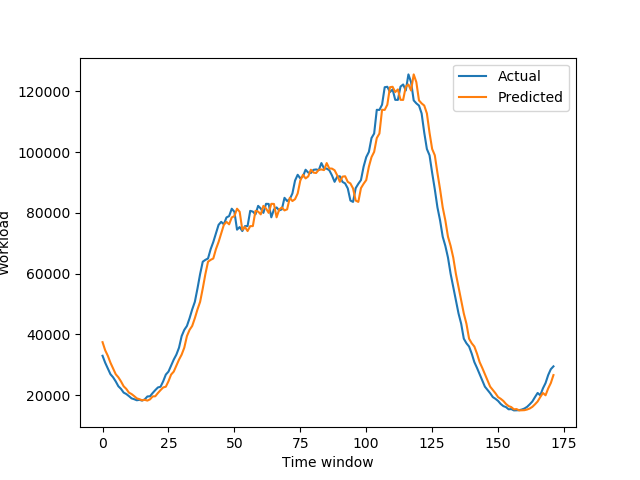
\includegraphics[width=\linewidth]{resources/baseline/naive_predictions_10.png}
      \caption{Naive prediction}
    \end{subfigure}
    \begin{subfigure}[b]{0.48\linewidth}
      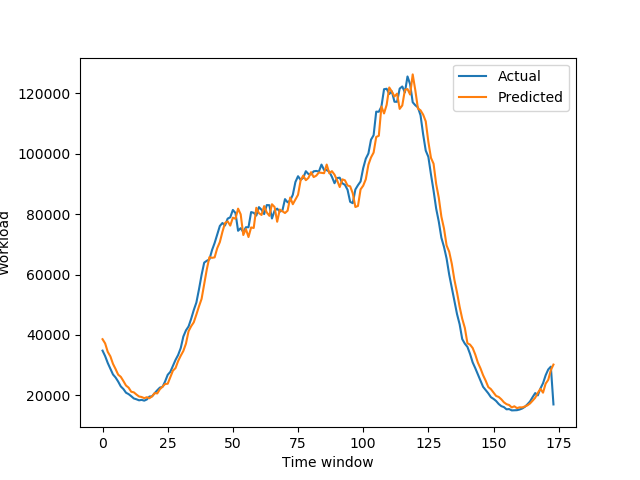
\includegraphics[width=\linewidth]{resources/baseline/arima_10.png}
      \caption{Arima prediction}
    \end{subfigure}
    \caption{Baseline predictions}
    \label{fig:baseline_pred}
  \end{figure}

  \subsubsection{ARIMA}
  ARIMA\cite{arima}, which stands for autoregressive integrated moving average, is a classic approach 
  to modelling timeseries. In order to apply this model we need to find appropiate values for its 
  parameters: p, q, d. 
  
  The value of d means the number of times the series needs to be differentiated
  in order to make it stationary. The series stationarity was checked using the augmented Dickey-Fuller 
  test\cite{Dickey-Fuller} which found the p-value to be 1.0902496274664773e-08. This is lower than 0.05, 
  the commonly used threshold, meaning we can set d to 0. 
  
  The partial autocorrelation plot was analyzed
  to set the autoregression parameter (p). From figure \ref{fig:arima_params} we can see that the significance
  region is confidently passed at 1, with a steep decline afterwards. The moving average parameter (q) is 
  approximated from the autocorrelation plot. It suggests a value of around 20 would be a good start. 
  After fitting ARIMA(1,0,20) the final 2 layers had P-value of 0.547 and 0.758 which meant that they were 
  not significant. After trying some values for q: 5,10,15,18 the best results were obtained on ARIMA(1,0,15)
  with 14263566.564, MAE: 3056.765, MAPE: 6.349.

  \begin{figure}
    \centering
    \begin{subfigure}[b]{0.4\linewidth}
      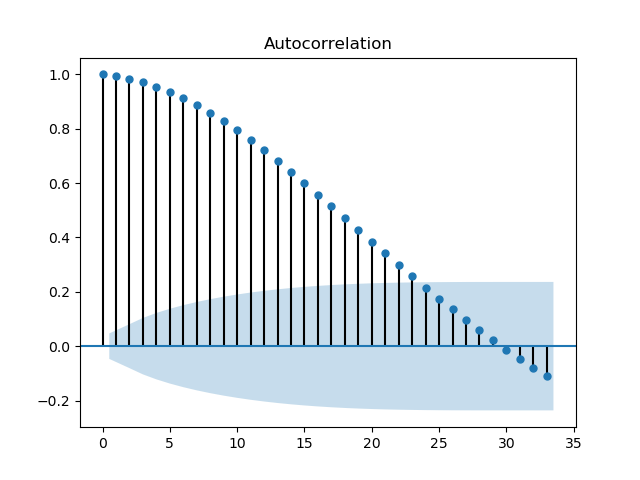
\includegraphics[width=\linewidth]{resources/baseline/arima_10_acf.png}
      \caption{Autocorrelation plot}
    \end{subfigure}
    \begin{subfigure}[b]{0.4\linewidth}
      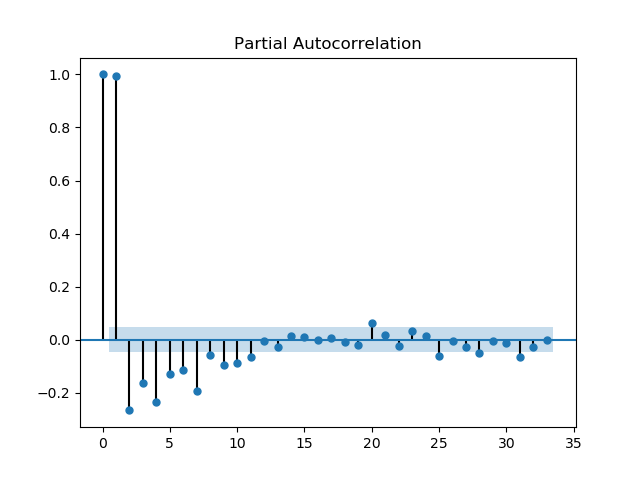
\includegraphics[width=\linewidth]{resources/baseline/arima_10_pacf.png}
      \caption{Partial autocorrelation plot}
    \end{subfigure}
    \caption{ARIMA params}
    \label{fig:arima_params}
  \end{figure}

  \subsection{Deep learning models}

  \subsubsection{MLP}
  After some manual experiments started with a MLP with 2 hidden layers (150, 100 neurons) and sliding window
  size of 24 (input size). 

  To find an optimal combination of batch size and epoch no a 2d grid search was performed \ref{fig:epoch_batch}.
  Batch size should ideally be a power of 2 for extra perfromance on GPU architectures, as some 
  experiments were ran on Google Colab. Lower batch size is more accurate but training is slower\cite{batch_size}.
  As expected the best MSE is obtained for the lowest batch size(4) however it does not drop significantly
  at 8, regardless of epochs no. The selection of epoch no is again a tradeoff between speed and accuracy. 
  We see a smaller no of epochs(50) performs poorly, while the difference between 100 and 250 is not that great,
  meaning that we can get a good approximation of a model using a batch size of 100.

  \begin{figure}
    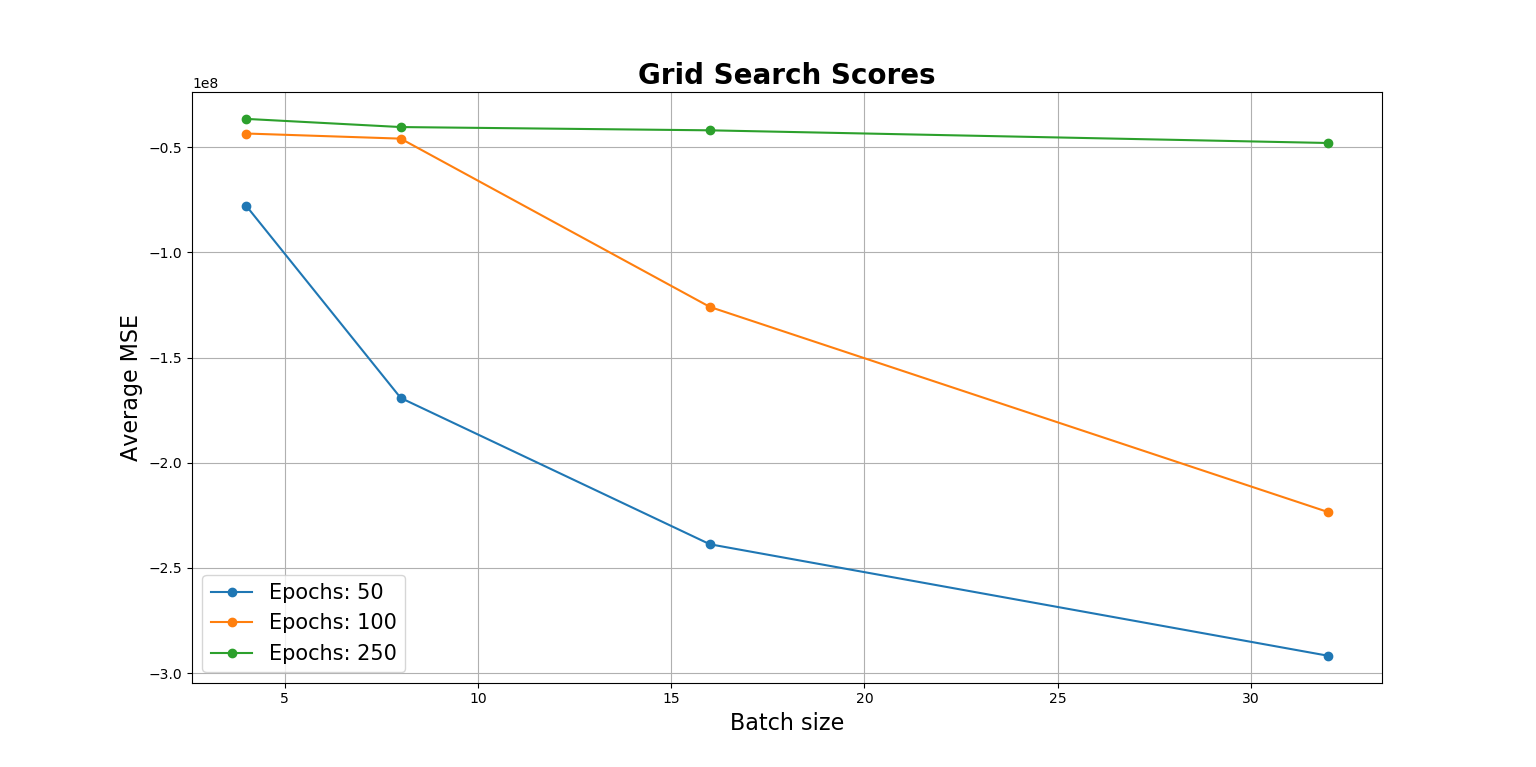
\includegraphics[width=\linewidth]{resources/mlp/epochs_batch.png}
    \caption{2d grid search for epoch no and batch size}
    \label{fig:epoch_batch}
  \end{figure}

  Some experiments were done with adding Dropout layers on different values (0.2, 0.1, 0.05) however it did 
  not improve performance. These are generally used to prevent overfitting, when the network is too big, the 
  data is scarce or training is done for too long\cite{dropout}, which was not the case for this experiment.

  Various optimizer and activation functions were tested. The Adadelta optimizer and the 
  relu activation were selected. A comprehensive grid search was performed for sliding window size and number 
  and content of hidden layers, of around 90 combinations. Some of the best performing are presented 
  in table \ref{tab:layers}.

  \begin{table}
    \caption{Selecting optimizer and activation. Scores are averaged MSE.}
    \begin{minipage}{.5\linewidth}
      \caption*{Optimizer}
      \centering
        \begin{tabular}{ll}
            RMSprop & 24734800\\
            Adadelta & 19291753\\
            Adagrad & 190604349\\
            Adam & 25828119\\
            Adamax & 29578706\\
            Nadam & 20400557
        \end{tabular}
    \end{minipage}%
    \begin{minipage}{.5\linewidth}
      \centering
        \caption*{Activation function}
        \begin{tabular}{ll}
            softmax & 4875804739\\
            softplus & 20314197\\
            softsign & 4034049993\\
            relu & 19571788\\
            tanh & 4175933232\\
            sigmoid & 3055609656\\
            linear & 20661311
        \end{tabular}
    \end{minipage}
  \end{table}

  \begin{table}
    \begin{center}
      \caption{MLP layers and size tuning}
      \label{tab:layers}
      \begin{tabular}{c|c|c}
        \textbf{Sliding window} & \textbf{Layers} & \textbf{MSE}\\
        \hline
        4 & (100, 50, 25, 20, 10) & 18889414\\
        4 & (10, 10, 10, 10, 10, 10) & 18935098\\
        4 & (100, 50, 50, 20, 10) & 18847516\\
        8 & (100, 50, 25, 20, 10) & 17044955\\
        8 & (150, 50, 50, 50, 50, 10) & 17216134\\
        8 & (50, 50, 50, 50) & 18394493\\
        16 & (10, 20, 30, 40, 50) & 18116299\\
        16 & (100, 20, 20, 20, 10) & 18466524\\
        16 & (10, 10, 10, 10, 10, 10, 10) & 18311036\\
      \end{tabular}
    \end{center}
  \end{table}

  \subsubsection{CNN}
  Firstly, a baseline model was selected through manual experimentation. This had the following structure:
  intput of size 20, a 1d convolutional layer, a maxpooling layer, a flatten layer, a dense layer of size 150 
  and the output layer. The same batch size, epoch no grid search was performed and it yielded similar results 
  to \ref{fig:epoch_batch}. This was followed by iterating the same optimizers and activation function in 
  order to select Adadelta and softplus. 

  \begin{table}
    \begin{center}
      \caption{CNN layers and size tuning}
      \label{tab:layers_cnn}
      \begin{tabular}{c|c|c}
        \textbf{Sliding window} & \textbf{Layers} & \textbf{MSE}\\
        \hline
        8 & (25, 10, 5) & 35385451\\
        64 & (100, 20, 10, 5) & 35012864\\
        128 & (100, 20, 10, 5) & 21086942\\
        128 & (300, 50) & 22287266\\
        128 & (10, 10, 10) & 23441869\\
        256 & (100,20,10,5) & 23783826\\
      \end{tabular}
    \end{center}
  \end{table}

  The main idea behind using a CNN model for this task is to pass a larger history window as input. 
  CNN layers build different filter that learn certain characteristics of the input data. They are well 
  suited for data which has a spatial relationship(like timeseries)\cite{cnn}.

  \subsubsection{CNN-LSTM Hybrid}
  This model was applied on a range of timeseries tasks by Lin et al.\cite{cnn_lstm}.
  The starting values for 
  some parameters were influenced by this research: 32 cnn filters, 1 lstm layer with 
  a couple hundred units.

  \begin{table}
    \begin{center}
      \caption{CNN-LSTM layers and size tuning}
      \label{tab:layers_cnn_lstm}
      \begin{tabular}{c|c|c}
        \textbf{Sliding window} & \textbf{LSTM layers} & \textbf{MSE}\\
        \hline
        144 & (20, 10, 5) & 51700082\\
        todo & todo & todo\\
      \end{tabular}
    \end{center}
  \end{table}


  \subsection{Experiment Results}

  Each of the most promising models were then trained again on all training data,
  for a larger number of epochs and repeated multiple times to account for the 
  random weight initialization. The best results were then compared to baselines
  and to eachother as seen in table \ref{tab:final_eval}.

  \begin{table}[h]
    \begin{center}
      \caption{Final results}
      \label{tab:final_eval}
      \begin{tabular}{c|c|c|c|c|c}
        \textbf{Dataset} & \textbf{Naive} & \textbf{ARIMA} & \textbf{MLP} & \textbf{CNN} & \textbf{CNN-LSTM} \\
        \hline
        Jp10 & 20233320 & 15289199 & 8591086 & 11709317 & 7252806 \\
        Jp15 & 87883950 & 56662039 & 31042348 & 35069911 & 57719162 \\
        De10 & 16789198 & 10318406 & 5180340 & 10526800 & todo \\
        De15 & 77481580 & 43398336 & 17276322 & 35485149 & todo \\
      \end{tabular}
    \end{center}
  \end{table}

  \section{For article - REMOVE ME}
  \subsection{Data preparation}
  The raw data used for this experiment is a wikipedia trace for 12 days in september 2007\cite{wikidata}. From this a subset of requests was extracted as separate datasets: all requests to Japanese and German wikipedia respectively. 
The subsets were selected in order to compare results with Kim et al.\cite{CloudInsight} which used the same data. Another reason for extracting subsets it's that the amount of data after preparation is the same as what we would extract from the global trace, given it's the same time range,
but processing is much faster.

In order to turn a web request log file into a supervised dataset the following steps were taken: 
\begin{itemize}
\item extract timestamps of all requests for a country (e.g. all lines matching ja.wikipedia)
\item create buckets which contain the number of requests in a time interval
\item iterate over the buckets using the sliding window technique, described below
\end{itemize}

The starting point for the sliding window technique\cite{sliding_window} is a time series $(t_1, t_2, .., t_{size})$ where $t_i$ is the number of requests in the i-th bucket. Training instances are then generated with input $(t_{i}, t_{i+1}, ... t_{i+n-1})$ and output $(t_{i+n+1})$, where n is the size of the sliding window. This process starts at i = 1 and is incremented by 1 until i = size - n + 1. The predicted value is $t_{i+n+1}$ instead of $t_{i+n}$ because a scaler using this model would need to have a buffer window during which to deploy the services.

\begin{figure}
  \centering{
    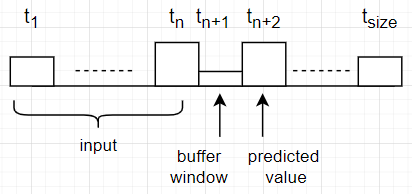
\includegraphics[scale=0.48]{resources/data/prepare.png}
  }
  \caption{Sliding window technique}
  \label{fig:sliding_window}
\end{figure}

The size of the datasets before applying the sliding window are 111316009 requests for ja.wikipedia and 101917920 for de.wikipedia.


\subsection{Approach tex}
\subsubsection{Baseline models}
Two baseline models were applied: a naive approach and a classic timeseries model, ARIMA.
They were selected to verify if machine learning is at all useful for this problem
and if it can learn features not considered by simpler methods.

The naive approach just assumes that the predicted workload is the same 
as the last observed workload. No proactive scaler could use this model 
as the predicted change in traffic is always 0, but we must check if the 
proposed models perform better than doing no prediction at all.

ARIMA\cite{arima}, which stands for autoregressive integrated moving average, is a classic approach
to modelling timeseries. It has been selected because it has been applied to 
workload prediction before\cite{arima_prediction} and because it combines 
multiple simpler models into a performant one. Autoregressive models
make predictions based on previous observations while moving average models 
use recent forecast errors. The integrated part indicates whether the 
series needs to be differentiated, and how many times.


\subsection{Deep Learning Models}

We have chosen in this investigation to apply the following deep learning architectures: MLP, CNN, CNN-LSTM hybrid, all of which have been shown to perform well on timeseries tasks \cite{dl_ts}\cite{dlts_book}\cite{cnn_lstm}. Also, deep learning has constantly outperformed classic methods in prediction tasks\cite{dlrev}. 

The selected models all have advantages and drawbacks among each other regarding training speed, the amount of data required to produce good answers and the tuning of the size of the sliding window to capture relevant recent information.

\subsubsection{MLP}
MLPs are quintessential deep learning models which although efficient in their own right also serve as baselines for more sophisticated architectures\cite{mit_dlbook}. It is made up out of an input layer, a number of hidden layers and an output layer, linked by weights which are learned through the backpropagaton algorithm. While a MLP with one hidden layer is theoretically sufficient to represent any function, that layer may be too large and training could be affected by overfitting, therefore deeper models can help reduce the generalization error\cite{neural_smithing}. 

This model has been selected to check whether looking at a smaller sliding window, without taking into account further historical dependencies, achieves satisfactory results.

\subsubsection{CNN}
CNNs are specialized in dealing with data that has a grid-like topology such as images(2d) or timeseries(1d)\cite{mit_dlbook}. They have the ability to learn filters which assign importance to some aspects of the input data, which is done by the convolutional layers. Another type of layer they usually contain are the pooling layers which reduce the spatial size of the convolved features and make the representation invariant to small translations in input.

CNN has been tested in this experiment because it looks like a natural fit for a timeseries problem given its assumed spatial dependencies. CNNs can extract only the important features of the input, therefore they can efficiently work with a larger sliding window, and take into account more recent measurements when making a prediction. 

\subsubsection{CNN-LSTM Hybrid}
This model was applied on a range of timeseries tasks by Lin et al.\cite{cnn_lstm} and was shown to outperform both CNN and LSTM baselines.

Recurrent Neural Networks are Neural Networks that take into account the outcome of previous predictions while making the current one\cite{mit_dlbook}. LSTM, Long Short-Term Memory, networks are an improvement over RNNs in the sense that they are better at capturing long-term dependencies\cite{lstm}.

This model has been chosen because it combines the ability of CNNs to extract salient features from raw timeseries data with the capability of LSTMs to find long range dependencies and historical trends.

\section{Experiments tex remove me}
In this section we will describe the experiments that we conducted, their results and a comparative analysis of these results.

We have chosen for the tuning phase the Japanese wiki dataset described in section 4 because besides that fact that includes significant patterns, it also has some interesting irregularities, like a huge spike which is not repeated. This dataset was also used by Kim et al.\cite{CloudInsight} and we intend to compare to obtained results.

\subsection{Settings}
The selected time window for tuning is 10 min, because it seemed a reasonable prediction time to allow a scaler to spin out new instances based on data from netflix\cite{scryer}. A plot of this dataset can be seen in figure \ref{fig:jp10}.

\begin{figure}
	\centering{
	   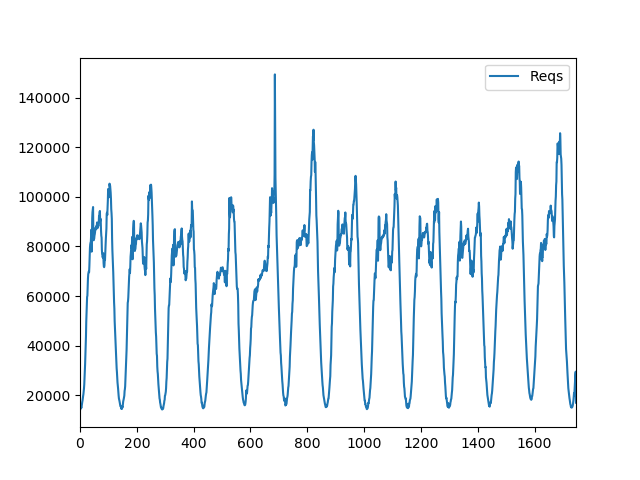
\includegraphics[scale=0.45]{resources/data/jp10.png}
	}
	\caption{Japanese wiki dataset, grouped by number of requests in 10 minute windows}
	\label{fig:jp10}
\end{figure}

After creating the 10min buckets we end up with 1747 data points. They are split into training and testing with a ratio of 0.9.

The validation method is k-fold Cross-Validation\cite{kfold} with k = 3, which means splitting the training dataset into k equal parts, perform training on k - 1 and evaluation on the part left out and then repeat this process until evaluation was done on each of the parts. The instances themselves are not shuffled inside the partitions, as their ordering is significant for LSTM models. 

K-fold validation estimates how well a model will perform on previously unseen data and offers a less biased skill estimation than the classic train/test validation method.
We do not want to see the testing data while tuning the model, because then the evaluation would influence the training process.

\subsection{Naive baseline}
The naive baseline obtains the following results, 20.2 mil MSE, 3577.8 MAE and 7.1 MAPE. This illustrates the fact that although the MAPE score would classify it as a very good predictor it does not do anything useful and the proposed models should achieve better results.

\subsection{ARIMA}
In order to apply the ARIMA model we need to find appropiate values for its parameters: p, q, d. The value of d means the number of times the series needs to be differentiated in order to make it stationary. The series stationarity was checked using he augmented Dickey-Fuller test\cite{Dickey-Fuller} which found the p-value to be $1.09e-08$. This is lower than 0.05, the commonly used threshold, meaning we can set the d to 0.

The partial autocorrelation plot was analyzed to set the autoregression parameter(p). From figure \ref{fig:pacfplot} we can see that the significance region is confidently passed at 1, with a steep decline afterwards. The moving average parameter(q) is approximated from the autocorrelation plot. It suggests a value of around 20 would be a good start. After fitting ARIMA(1,0,20) the final 2 layers had p-value of 0.547 and 0.758 which meant that they were not significant. 

After trying some values for q: 5, 10, 15, 18, illustrated in table \ref{tab:arima_sesults}, the best results were obtained on ARIMA(1, 0, 15) with 14.2mil MSE, 3056.7 MAE and 6.3 MAPE.

\begin{figure}
    \centering{
    	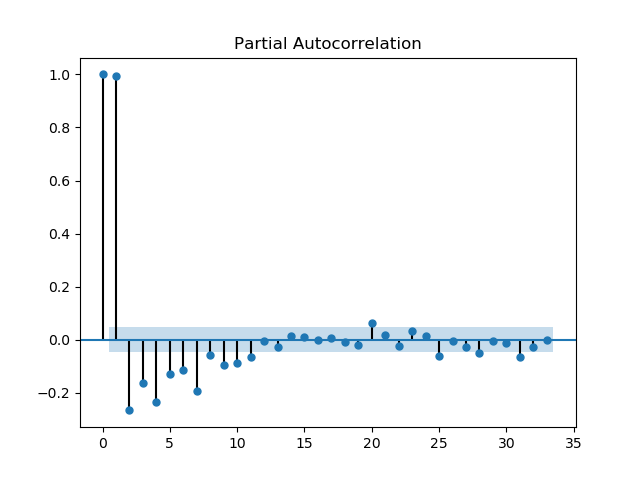
\includegraphics[scale=0.45]{resources/baseline/arima_10_pacf.png}
    }
    \caption{Partial autocorrelation plot (for ARIMA)}
    \label{fig:pacfplot}
\end{figure}

\begin{figure}
    \centering{
    	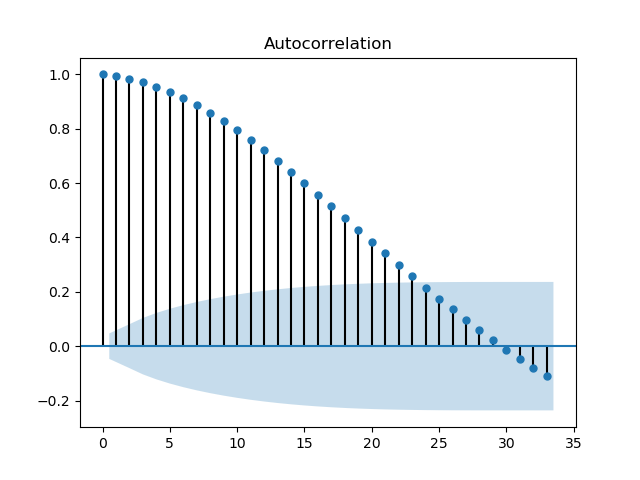
\includegraphics[scale=0.45]{resources/baseline/arima_10_acf.png}
    }
    \caption{Autocorrelation plot (for ARIMA)}
    \label{fig:acfplot}
\end{figure}


\begin{table}[htbp]
\caption{ARIMA tuning}
\begin{center}
\begin{tabular}{|c|c|c|}
\hline
p,d,q & MSE & prediction time \\
\hline
1,0,5 & 16.3m & 0.4s\\
\hline
1,0,10 & 15.3m & 9.6s\\
\hline
1,0,15 & 15.2m & 31s\\
\hline
1,0,18 & 15.3m & 71s\\
\hline
\end{tabular}
\label{tab:arima_sesults}
\end{center}
\end{table}

\subsection{MLP}

\subsubsection{Settings}
After some manual experiments we started with a MLP with 2 hidden layers (150, 100 neurons) and a sliding window size of 24 (input size). To find an optimal combination of batch size and epoch no a 2d grid search was performed, figure \ref{fig:epochs_batch_scaled}. Batch size should ideally be a power of 2 for extra performance on GPU architectures, as some experiments were ran on Google Colab's cloud GPU. Lower batch size is more accurate but training is slower\cite{batch_size}. As expected the best MSE is obtained for the lowest batch size(4) however it does not drop significantly at 8, regardless of epochs no. The
selection of epoch no is again a trade-off between speed and accuracy. We see a smaller no of epochs(50) performs poorly, while the difference between 100 and 250 is not that great,
meaning that we can get a good approximation of a model using a batch size of 100.

Some experiments were done with adding Dropout layers on different values (0.2, 0.1, 0.05) however it did not improve performance. These are generally used to prevent over-fitting, when the network is too big, the data is scarce or training is done for too long\cite{dropout}, which was not the case for this experiment.

\begin{figure}
    \centering{
    	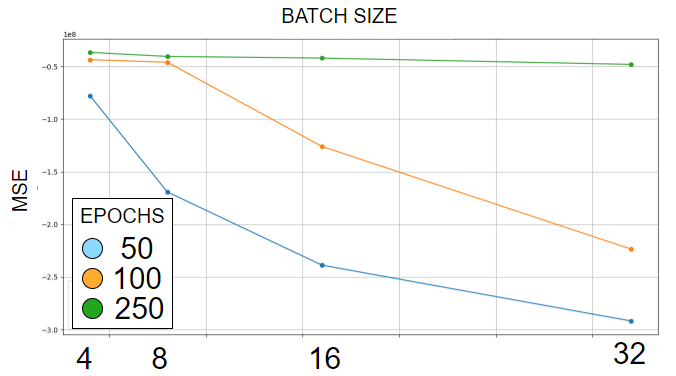
\includegraphics[width=\linewidth]{resources/mlp/epochs_batch_scaled.png}
    }
    \caption{Grid search for epoch no and batch size}
    \label{fig:epochs_batch_scaled}
\end{figure}

Various optimizer and activation functions were tested. The Adadelta optimizer and the relu activation were selected. ReLU is also the default recommendation\cite{mit_dlbook} for modern neural networks, because it is non-linear while preserving many advantages of linear functions that make them generalize well. Although the ADAM optimizer is widely used in research there is no consensus on which is the optimal one\cite{mit_dlbook} therefore we chose Adadelta which in our experiments performed better (19.2m vs 25.8m MSE).

A comprehensive grid search was performed for sliding window size and number and content of hidden layers, of around 90 combinations. Some of the best performing are presented in table \ref{tab:mlp_tune}.

\begin{table}[htbp]
\caption{MLP tuning}
\begin{center}
\begin{tabular}{|c|c|c|}
\hline
Sliding window & Hidden layers & MSE \\
\hline
4 & (100, 50, 25, 20, 10) & 18.8m\\
\hline
4 & (100, 50, 50, 20, 10) & 18.8m\\
\hline
8 & (100, 50, 25, 20, 10) & 17.0m\\
\hline
8 & (150, 50, 50, 50, 50, 10) & 17.2m\\
\hline
8 & (50, 50, 50, 50) & 18.3m\\
\hline
16 & (10, 20, 30, 40, 50) & 18.1m\\
\hline
16 & (100, 20, 20, 20, 10) & 18.4m\\
\hline
\end{tabular}
\label{tab:mlp_tune}
\end{center}
\end{table}

\subsubsection{Results}
The final parameters for the proposed MLP model are: Adadelta optimizer with ReLU activation function, a sliding window of size 8 with 5 hidden layers of size: 100, 50, 25, 20, 10.

\subsection{CNN}

\subsubsection{Settings}
Firstly, a baseline model was selected through manual experimentation. This had the following structure: input of size 20, a 1d convolutional layer, a maxpooling layer, a flatten layer, a dense layer of size 150 and the output layer. The same batch size, epoch no grid search was performed and it yielded similar results to \ref{fig:epochs_batch_scaled}. This was followed by iterating the same optimizers and activation function in 
order to select Adadelta and softplus.

A grid search was again performed in order to find out the optimal sizes for sliding window, hidden layers and their neurons (see table \ref{tab:cnn_tune}). This proves our assumption that CNNs can extract better features from larger sliding window as best results were obtained with a window of 128 as opposed to 8 for MLPs.

\begin{table}[htbp]
\caption{CNN tuning}
\begin{center}
\begin{tabular}{|c|c|c|}
\hline
Sliding window & Hidden layers & MSE \\
\hline
8 & (25, 10, 5) & 35.3m\\
\hline
64 & (100, 20, 10, 5) & 35.0m\\
\hline
128 & (100, 20, 10, 5) & 21.0m\\
\hline
128 & (300, 50) & 22.2m\\
\hline
128 & (10, 10, 10) & 23.4m\\
\hline
256 & (100, 20, 10, 5) & 23.7m\\
\hline
\end{tabular}
\label{tab:cnn_tune}
\end{center}
\end{table}

\subsubsection{Results}
The parameters selected for the CNN model are: Adadelta optimizer, softplus activation function, a window of size 128 and 4 hidden layers of size: 100, 20, 10, 5.

\subsection{CNN-LSTM Hybrid}

\subsubsection{Settings}
The starting values for some parameters were influenced by the research done by Lin et al.\cite{cnn_lstm}: a convolutional layer with 32 cnn filters, a max pooling layer, a lstm layer with a couple hundred units. In order to feed the output of the convolutional layers into the LSTM layer the input was broken into multiple sequences. This provided the time dimension which LSTM input shape specifies, as the sequences are arranged in a temporal order.

A similar search as in previous sections was performed to select Adadelta optimizer and ReLU activation function.

While searching for the size of the LSTM layer we observed a trend where error value would become very large after a couple of epochs, of approximatevely $1.7 \cdot 10^{27}$. This might be linked with gradient explosion\cite{mit_dlbook} which causes a network to become unstable because of an increase in the number or values of the gradients with which the inputs are multiplied. Therefore, we applied a common solution, to rescale elements in a gradient vector if their norm exceeds 1, which has solved the issue.

A search was then performed for different combinations of sliding window size, cnn sequences and lstm units, which can be observed in table \ref{tab:cnn_lstm_tune}.

\begin{table}[htbp]
\caption{CNN-LSTM tuning}
\begin{center}
\begin{tabular}{|c|c|c|}
\hline
Input shape & LSTM Units & MSE \\
\hline
(20, 15) & 500 & 246.0m\\
\hline
(16, 16) & 150 & 98.3m\\
\hline
(12, 12) & 750 & 93.6m\\
\hline
(12, 12) & 500 & 61.8m\\
\hline
(8, 8) & 500 & 370.1m\\
\hline
\end{tabular}
\label{tab:cnn_lstm_tune}
\end{center}
\end{table}

\subsubsection{Results}
From the previously described experiments we selected the following parameters for this model: Adadelta optimizer, ReLU function, (12, 12) input shape with 500 lstm units.

\subsection{Analysis}
Each of the most promising models were then trained again on all training data, and evaluated on the testing data, which was unseen during tuning. This measurement has been repeated multiple times to account for the random weight initialization. The best results were then compared to baselines and to each other as seen in table \ref{tab:final_results}.

\begin{table}[htbp]
\caption{Final results}
\begin{center}
\begin{tabular}{|c|c|c|c|c|c|}
\hline
DataSet & Naive & ARIMA & MLP & CNN & CNN-LSTM \\
\hline
Jp10& 20.2m & 15.2m & 8.5m & 11.7m & todo\\
\hline
Jp15 & 87.8m & 56.6m & 31.0m & 35.0m & todo\\
\hline
De10 & 16.7m & 10.3m & 5.1m & 10.5m & todo\\
\hline
De15 & 77.4m & 43.3m & 17.2m & 35.4m & todo\\
\hline
\end{tabular}
\label{tab:final_results}
\end{center}
\end{table}


  \newpage
  \bibliography{bibliography}{}
  \bibliographystyle{plain}
\end{document}